\section{Caos en Redes Neuronales}
\label{sec:RNA}

El problema del caos en las redes neuronales ha recibido mucha atención recientemente \cite{Yang2003}.
Las actividades en este campo pueden ser divididas en tres categorías:
\begin{itemize}
	\item Estudio experimental del comportamiento aperiódico observado en una sola neurona perturbada o en un pequeño ensamble de neuronas.
	\item Estudio del comportamiento temporal complejo del cerebro y los posibles	roles del caos en el procesamiento de la información.
	\item Estudio de las rutas al caos y las propiedades de los atractores caóticos en en modelos de redes neuronales.
\end{itemize}

Las redes neuronales artificiales proveen soluciones efectivas a problemas en diversos campos, en particular, pueden servir como generadores de señales caóticas.
Las aplicaciones de señales caóticas son muy diversas, pero en este caso son especialmente atractivas ya que en los algoritmos de aprendizaje se realiza una búsqueda aleatoria, entonces un generador neuronal de caos puede ser parte de la red neuronal determinística que se está entrenando.

\subsection{El Modelo de Hopfield}

Una de las piedras fundamentales para el reciente renacimiento en el campo de las redes neuronales fue el modelo asociativo propuesto por Hopfield en 1982.
La aproximación de Hopfield es un enfoque teórico para pensar ensambles entre unidades de cómputo \cite{Weise2009}.

El perceptrón multicapa es una Red Neuronal Artificial (RNA) formada por capas de neuronas.
Las neuronas pueden pertenecer a la capa de entrada, capas ocultas o capa de salida.
Estas neuronas no poseen memoria, por lo que su salida depende del estado de sus entradas en el instante actual (no tienen retardo), además, como el nombre de sus capas lo sugiere, las conexiones son unidireccionales y jerárquicas.
Es por esto que la matriz de pesos tiene solo algunos valores distintos de cero, no hay conexiones hacia atrás, ni en la misma capa, ni sobre la misma neurona, ni salteándose capas.
En la Figura \ref{fig:PerceptronSimple} se ve un ejemplo para un perceptrón pequeño y su matriz de pesos.

\begin{figure}
	\centering
	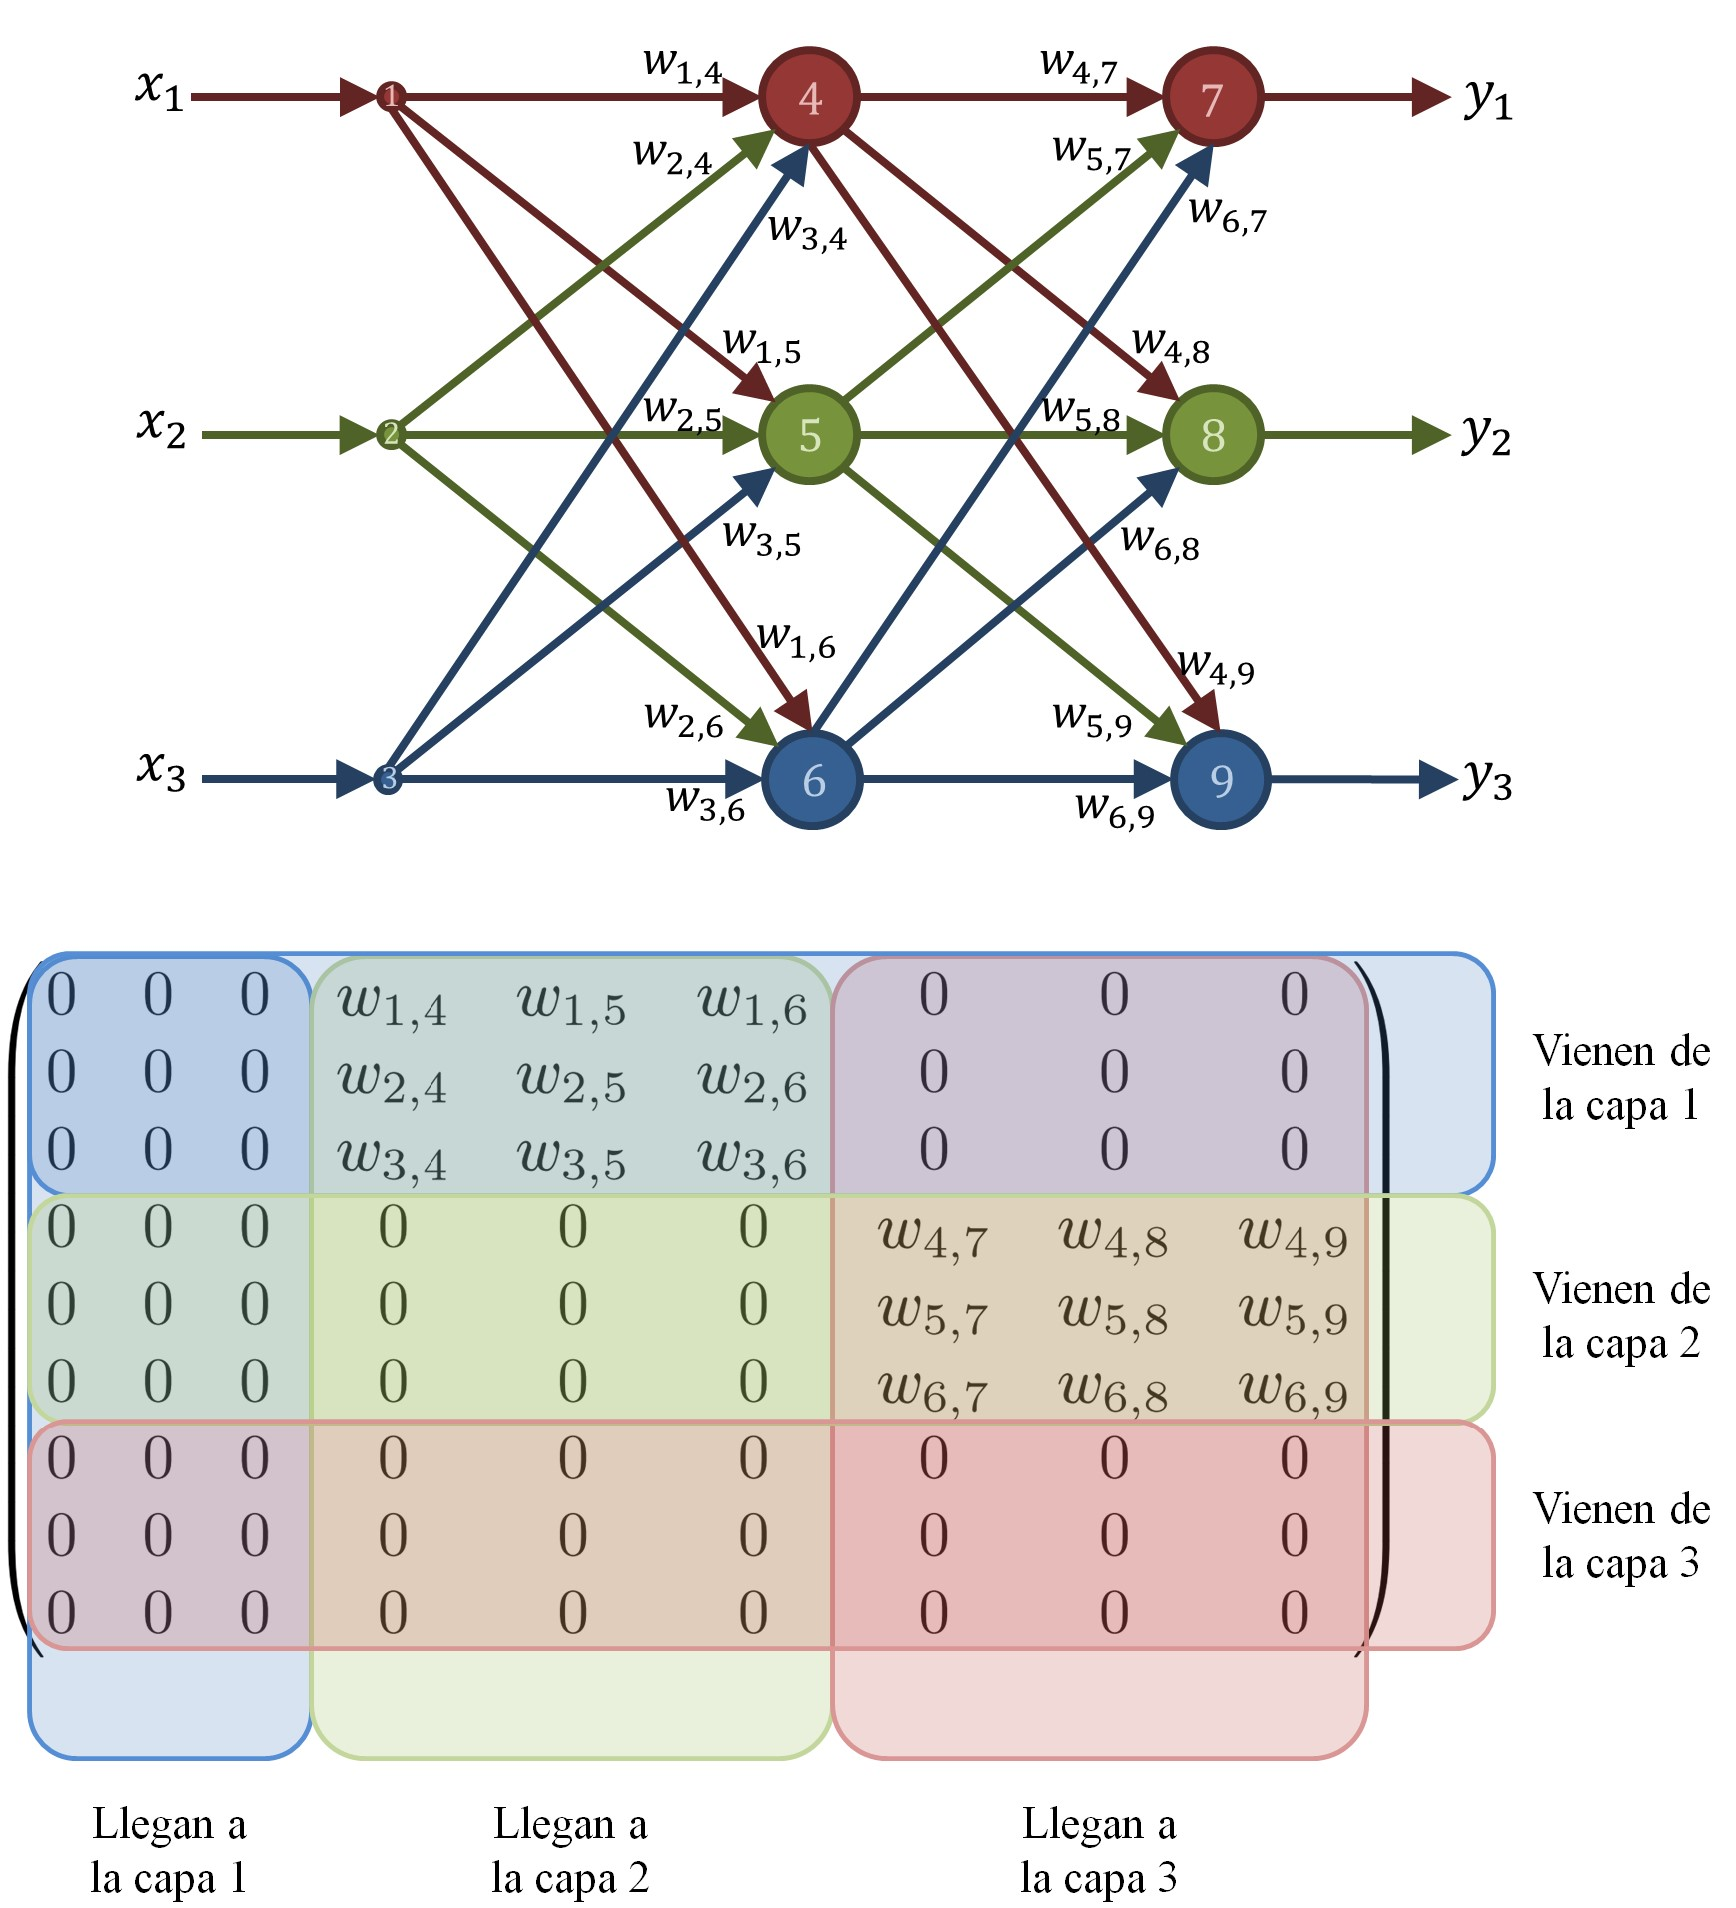
\includegraphics[width=.75\columnwidth]{PerceptronSimple}\\
	\caption{Perceptrón multicapa y matriz de pesos asociada. Puede verse que la topología de la red y la configuración de la matriz de pesos son biunívocas.}\label{fig:PerceptronSimple}
\end{figure}

Al contrario de los perceptrones multicapa, los sistemas adaptativos y los mapas auto-organizados, las redes de Hopfield sí tienen realimentación entre neuronas.
Este tipo de arquitectura tiene como campo principal de aplicación la optimización de procesos.
Se basa en el planteamiento de una memoria asociativa, es decir que el estado actual de una neurona depende de su historia y de la de las neuronas asociadas a ella; se hace necesario entonces definir una función de energía.
Además, se destaca la facilidad de implementación en FPGA y VLSI.

Esta red recurrente se basa en almacenar información en un sistema que presenta una configuración dinámica estable, es decir, se plantea como una memoria asociativa o memoria direccionable por contenido.
Intuitivamente, la idea de Hopfield es localizar cada patrón que se requiere almacenar a la red en el fondo de un valle de la función de energía.
Se parte de un determinado estado inicial (información de partida) tras lo cual se deja evolucionar el sistema hasta llegar a un estado estable.
Este estado estable será el patrón que se corresponde con el estado inicial (reconocimiento de patrones).

Hopfield, en su trabajo destaca tres diferencias con el perceptrón multicapa:
\begin{itemize}
		\item Su modelo incluye realimentaciones, que son fundamentales en su modo de funcionamiento.
		\item La elección de la arquitectura del perceptrón multicapa se realiza en forma arbitraria.
		\item El perceptrón multicapa funciona de manera síncrona, es decir, todas las neuronas cambian al mismo tiempo. La red de Hopfield permite un funcionamiento tanto síncrono como asíncrono, aunque el funcionamiento asíncrono es el más habitual en las neuronas biológicas.
\end{itemize}

El grafo de la red cambia con respecto al perceptrón multicapa, la representación no es la de un grafo separable por capas con conexiones hacia adelante, sino la de un grafo completo como se ve en la Figura \ref{fig:RedHopfield}.
\begin{figure}
	\centering
	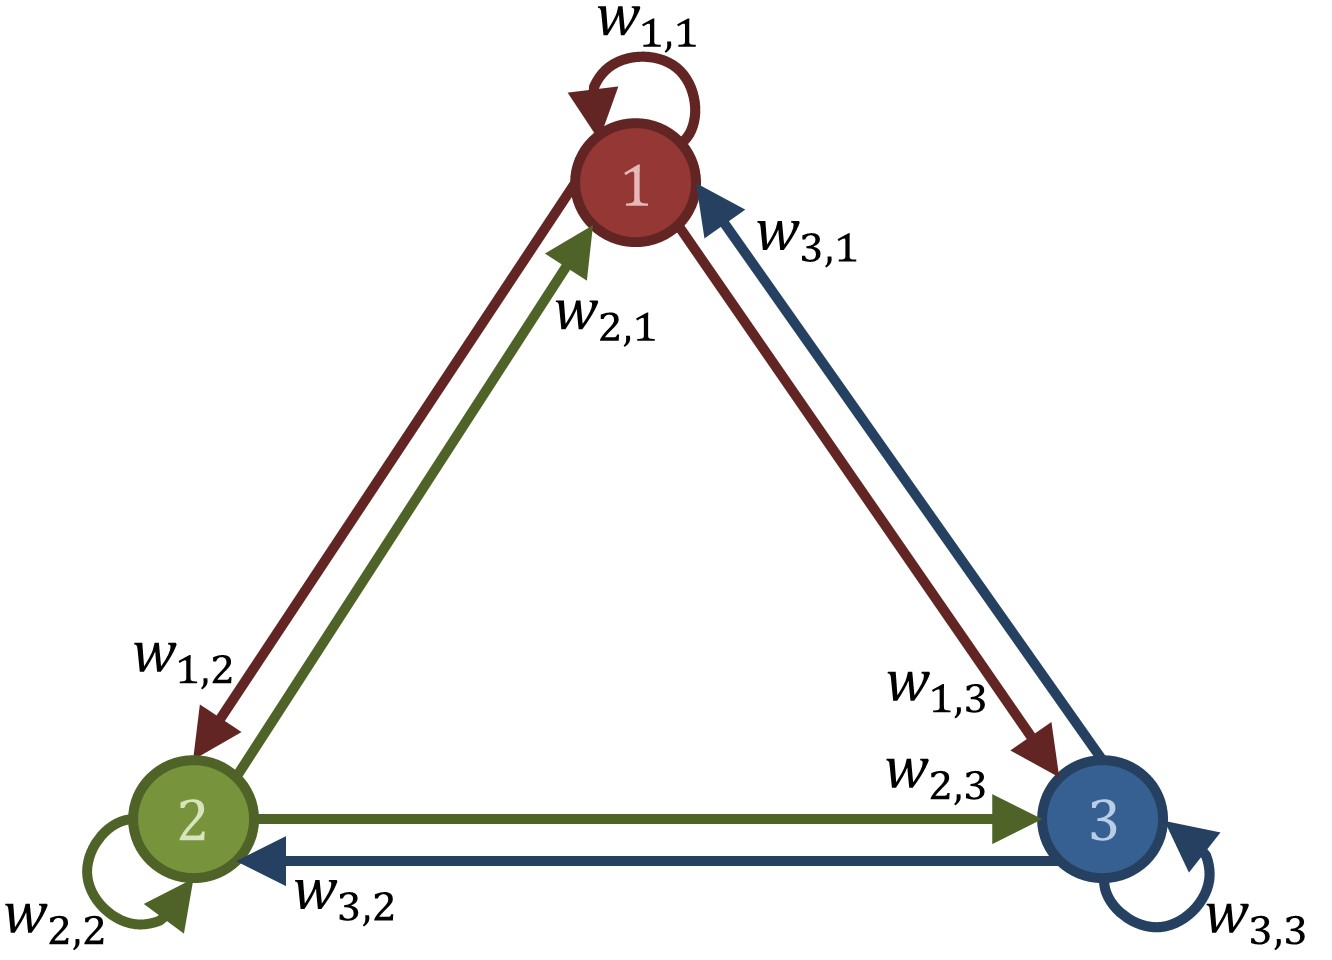
\includegraphics[width=.5\columnwidth]{RedHopfield}\\
	\caption{Red de Hopfield. Ahora, la matriz de pesos tiene todos sus valores permitidos.}\label{fig:RedHopfield}
\end{figure}

\subsection{Estudio de la RNA en Función de un Parámetro}

La red neuronal usada tiene siguiente el modelo de tiempo continuo:
\begin{eqnarray}\label{eq:ModTiempCont}
\dot{u} = -u + W \cdot f(u); \; u \in \mathbb{R}^3
\end{eqnarray}
en donde $u$ es un vector de tres dimensiones, $W$ es la matriz de pesos y $f$ es la función de activación
\begin{eqnarray}\label{eq:uWf}
u =
\left( \begin{array}{c}
x\\
y\\
z\\
\end{array} \right)
; \;
W =
\left( \begin{array}{ccc}
w_{1,1} & w_{1,2} & w_{1,3}\\
w_{2,1} & w_{2,2} & w_{2,3}\\
w_{3,1} & w_{3,2} & w_{3,3}
\end{array} \right)
; \;
f =
\left( \begin{array}{c}
\arctan x\\
\arctan y\\
\arctan z\\
\end{array} \right)
\end{eqnarray}

Las Ecuaciones \ref{eq:uWf} se corresponden con el diagrama de la Figura \ref{fig:RedHopfield}.
De la ecuación que se corresponde con una red de Hopfield de memoria diferencial.
No disponemos de computadoras analógicas, por lo que el sistema debe ser convertido a tiempo discreto.
Aunque el paquete de programas Matlab incluye rutinas para el cálculo de ecuaciones diferenciales, perdemos el control de paso de tiempo necesario para calcular el exponente de Lyapunov con el método descripto en la Sección \ref{secMLE}.
Por lo tanto, se emplea la aproximación de Euler de primer orden, en donde la derivada se aproxima con un trapecio de base $\Delta t$.
%
\begin{eqnarray}\label{eq:EulerRNA}
	\dfrac{u_{n+1}-u_n}{\Delta t} \approx \dot{u}_n &=& -u + W \cdot f(u_n) \Rightarrow\\ \nonumber
	\Rightarrow u_{n+1} &=& (1 - \Delta t)u_n + \Delta t W \cdot f(u_n)\\ \nonumber
						 &=& Gu_n + \Omega f(u_n)
\end{eqnarray}

En la Figura \ref{fig:EulerRNA} se muestra el diagrama de la red neuronal diseñada en tiempo discreto.
Sus coeficientes dependen del paso de tiempo.
Este sistema se aproxima al de tiempo continuo en el límite $\Delta t \rightarrow 0$, se verificó que el sistema converge al planteado.
Pudo verse que con $\Delta t = 1$ y $\Delta t = 0,1$ las soluciones en el espacio de fases fueron las mismas, para hacer los cálculos se empleó $\Delta t = 0,01$.
%
\begin{figure}
	\centering
	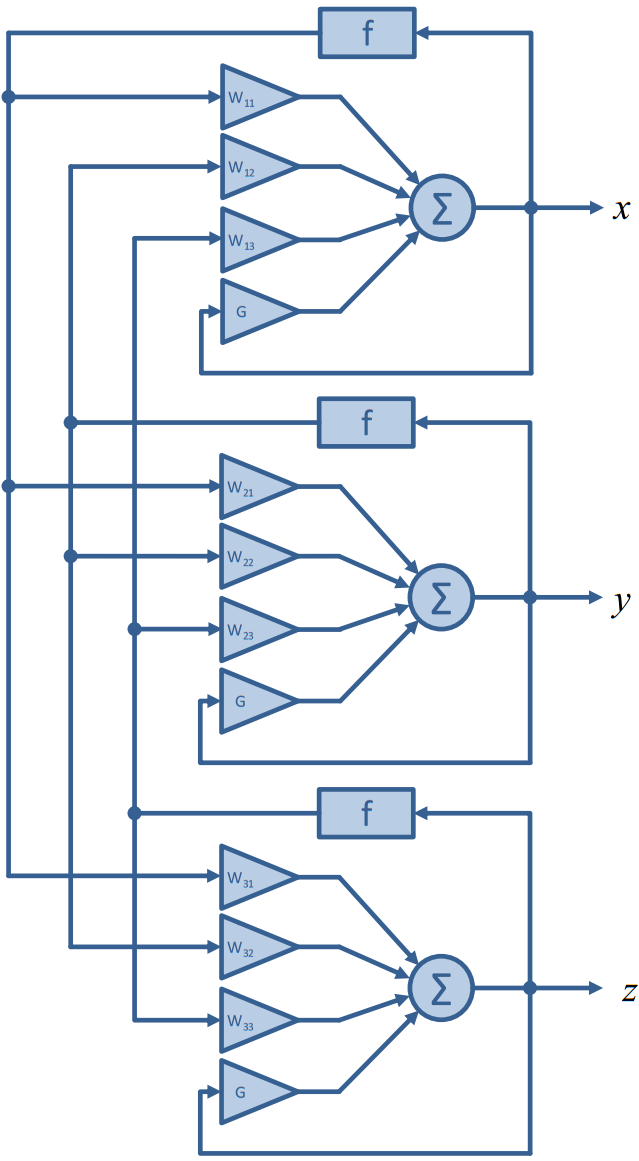
\includegraphics[width=.5\textwidth]{EulerRNA}\\
	\caption{Red utilizada. Se trata de una red de Hopfield tridimensional de memoria diferencial, el diseño está orientado a una posterior implementación en FPGA.}\label{fig:EulerRNA}
\end{figure}

Se barrió un parámetro (peso de un axón) para identificar la existencia de caos en función de éste.
Siguiendo a \cite{Yang2003} en donde se reporta una transición al caos en torno a un juego de parámetros, utilizamos la siguiente matriz de pesos:
%
\begin{eqnarray}\label{eq:matrizW}
W =
\left( \begin{array}{ccc}
2 & -1,2 & 0\\
1,9+p & 1,71 & 1,15\\
-4,75 & 0 &1,1
\end{array} \right)
\end{eqnarray}
%
en donde $p$ es el parámetro a barrer entre $-0,35$ y $0,55$ en pasos de $9\times 10^{-5}$.

Para cada valor del parámetro se le da condiciones iniciales al sistema $[1,68; -0,292; -3,47]$ y se lo deja evolucionar $800s$, esto es $200s$ más que el transitorio más largo reportado en \cite{Yang2003}, con esto nos aseguramos de descartar el transitorio y que el sistema se encuentra en régimen permanente.
Se calcula el MLE para $t \in (800;1~000]$.

De esta forma se genera la Figura \ref{fig:MLEvsp} en donde se muestra el MLE en función del parámetro.
Como es usual, el MLE no es una función suave, sino que es una función discontinua que presenta saltos abruptos en todo el dominio, sin embargo, se encontraron zonas de caos robusto frente al parámetro p en algunos intervalos, especialmente en $p \in (0,0223; 0,0791)$.
Esto significa que el caos persiste con una variación no infinitesimal del parámetro, esta zona es muy útil para implementaciones prácticas.
\begin{figure}
	\centering
	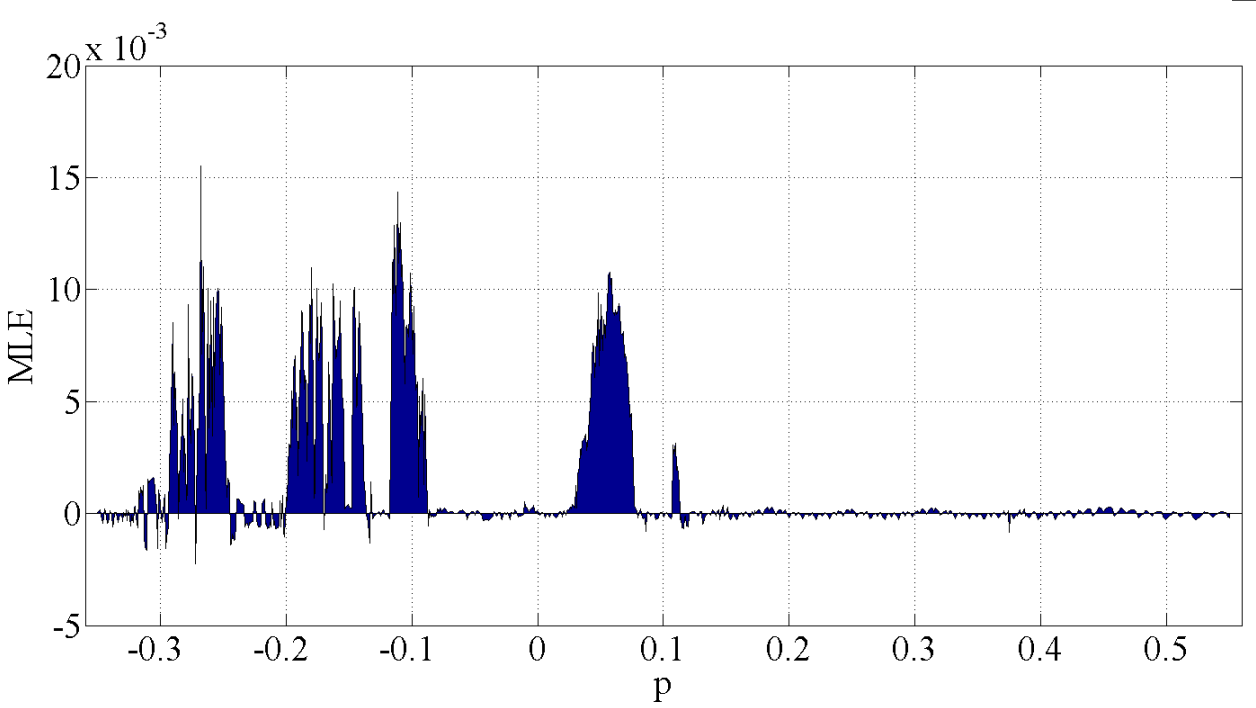
\includegraphics[width=1\columnwidth]{MLEvsp}\\
	\caption{MLE en función del parámetro p. Existe caos en toda la zona en la que es positiva.}\label{fig:MLEvsp}
\end{figure}

Para mostrar la transición al caos y la relación entre el MLE y el espacio de fases, se eligieron dos parámetros $p_1 = -0,2725$ y $p_2 = 0,268$, para $p_1$ el $MLE = -2,2\times10^{-3}$, para $p_2$ el $MLE = 1,55\times10^{-2}$.
Se muestra la trayectoria resultante para cada uno en la Figura \ref{fig:DetvsCaot}.
\begin{figure}
	\centering
	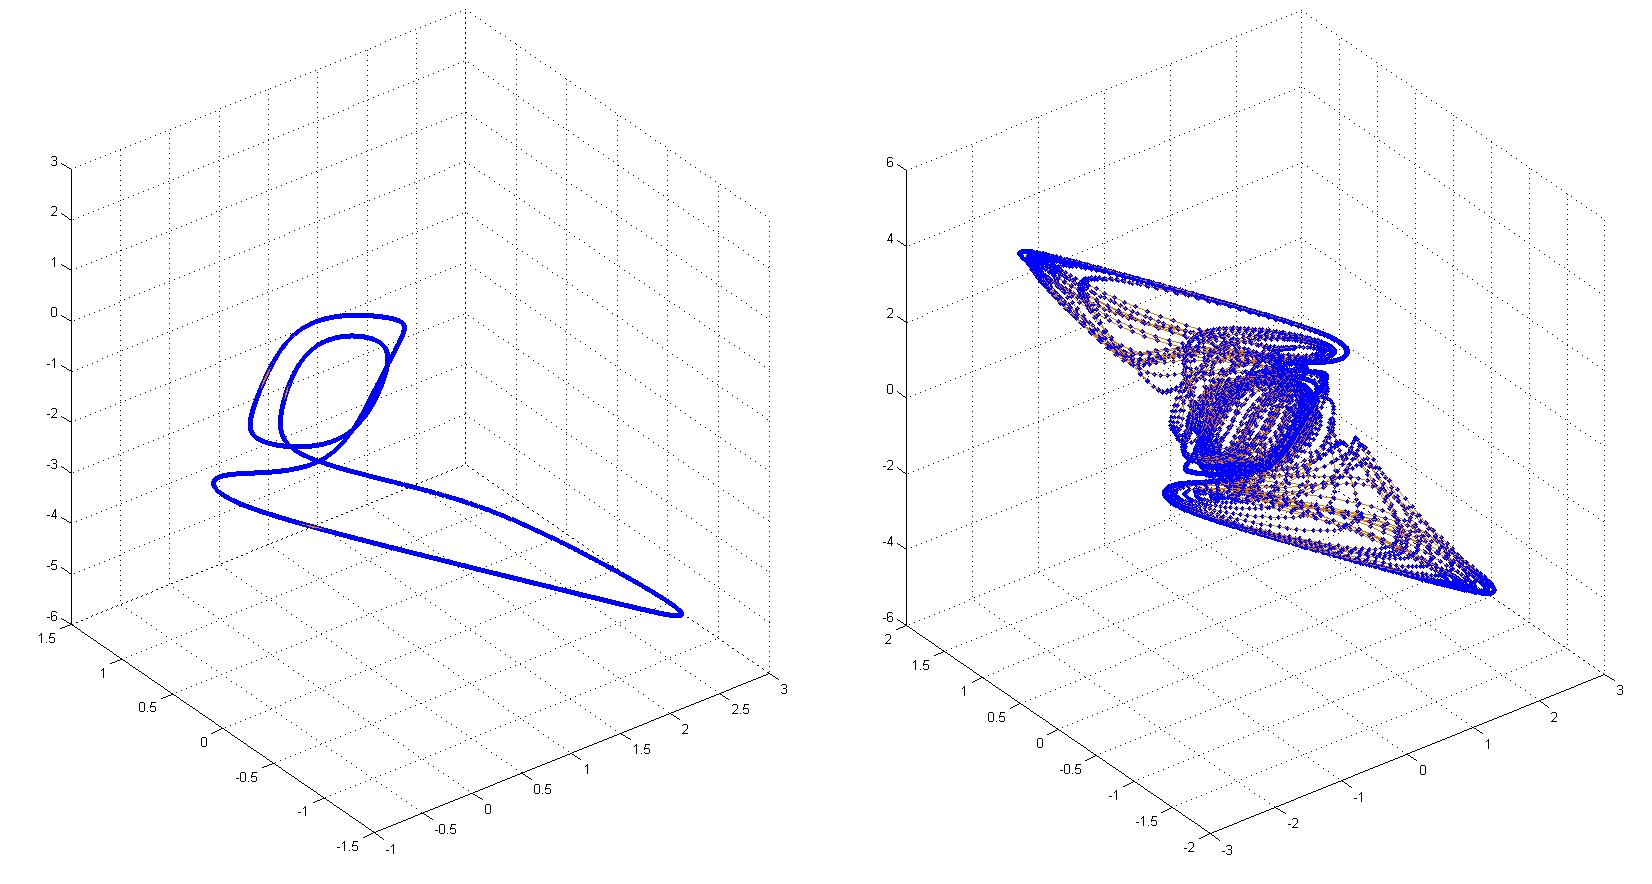
\includegraphics[width=1\columnwidth]{DetvsCaot}\\
	\caption{Dos trayectorias características del sistema en el espacio de fases. La trayectoria de la izquierda se corresponde con un $MLE < 0$ y la positiva con un $MLE > 0$.}
	\label{fig:DetvsCaot}
\end{figure}

Para el atractor caótico, dos trayectorias generadas a partir de condiciones iniciales muy cercanas deben, al cabo de un tiempo, separarse y oscilar en trayectorias distintas.
En la Figura \ref{fig:DosTrayectorias} puede verse este efecto.
\begin{figure}
	\centering
	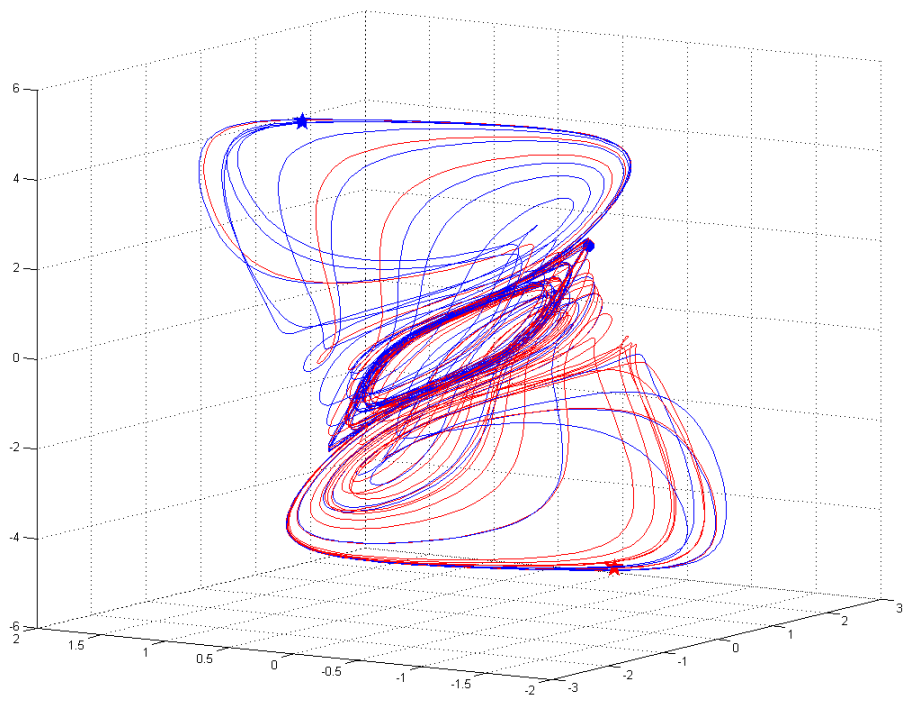
\includegraphics[width=.75\columnwidth]{DosTrayectorias}\\
	\caption{Dos trayectorias de la red de Hopfield para condiciones iniciales próximas.
		Las condiciones iniciales están marcadas con dos puntos grandes cerca del centro del atractor y los	valores después de $\Delta t = 3s$ con estrellas en ambos extremos de la figura.}
	\label{fig:DosTrayectorias}
\end{figure}